\section{Udvælgelse af gestik-par til at skrue op og ned for musikken}
\label{TestresultaterVolumen}
%
Udvælgelsen af hvilket gestik-par, der skal knyttes til at skrue op og ned for musikken foretages på baggrund af testpersonernes udsagn. I \fullref{app:TestresultaterVolumenDaarlig} analyseres testpersonernes respons i forhold til hvilke gestik-par de mindst kan lide og på baggrund af den analyse ekskluderes gestik-par 6, gestik-par 7 og gestik-par 8 fra yderligere undersøgelser. Dette medfører at udvælgelsen af hvilket gestik-par, der skal knyttes til at skrue op og ned kun foretages på gestik-par 1, gestik-par 2, gestik-par 3, gestik-par 4, gestik-par 5 og gestik-par 9.\blankline
%  
I nedenstående \autoref{tab:GestikParITopTreVolumen} fremgår samtlige testpersoners top tre rangering, hvor der ikke er taget forbehold for hvorvidt testpersonerne har inkluderet et gestik-par, som der på baggrund af \fullref{app:TestresultaterPauseDaarlig} er blevet ekskluderet.
%
\begin{table}[H]
	\centering
	\begin{tabular}{ | p{3cm} | p{3cm} | p{3cm} | p{3cm} |}
		\hline
		& 1. Plads & 2. Plads & 3. Plads \\ \hline
		Testperson 1 & Gestik-par 2 & Gestik-par 6 & Gestik-par 3 \\ \hline
		Testperson 2 & Gestik-par 4 & Gestik-par 5 & Gestik-par 6 \\ \hline
		Testperson 3 & Gestik-par 9 & Gestik-par 4 & Gestik-par 2 \\ \hline
		Testperson 4 & Gestik-par 3 & Gestik-par 1 & Gestik-par 2 \\ \hline
		Testperson 5 & Gestik-par 6 & Gestik-par 1 & Gestik-par 5 \\ \hline
		Testperson 6 & Gestik-par 3 & Gestik-par 4 & Gestik-par 8 \\ \hline 
		Testperson 7 & Gestik-par 2 & Gestik-par 5 & Gestik-par 3 \\ \hline
		Testperson 8 & Gestik-par 1 & Gestik-par 4 & Gestik-par 3 \\ \hline
		Testperson 9 & Gestik-par 9 & Gestik-par 1 & Gestik-par 4 \\ \hline
		Testperson 10 & Gestik-par 3 & Gestik-par 5 & Gestik-par 2 \\ \hline
		Testperson 11 & Gestik-par 3 & Gestik-par 4 & Gestik-par 8 \\ \hline
		Testperson 12 & Gestik-par 4 & Gestik-par 3 & Gestik-par 5 \\ \hline
		Testperson 13 & Gestik-par 3 & Gestik-par 2 & Gestik-par 1 \\ \hline
		Testperson 14 & Gestik-par 2 & Gestik-par 6 & Gestik-par 5 \\ \hline
		Testperson 15 & Gestik-par 3 & Gestik-par 4 & Gestik-par 9 \\ \hline
		Testperson 16 & Gestik-par 1 & Gestik-par 3 & Gestik-par 9 \\ \hline
		Testperson 17 & Gestik-par 2 & Gestik-par 9 & Gestik-par 3 \\ \hline
		Testperson 18 & Gestik-par 4 & Gestik-par 2 & Gestik-par 9 \\ \hline
	\end{tabular}
	\caption{Oversigt over samtlige testpersoners top tre i forbindelse med at ændre volumen.}
	\label{tab:GestikParITopTreVolumen}
\end{table}
\noindent
%
%
Få at få et overblik over hvor ofte de syv forskellige gestik-par individuelt indgår på enten en første, anden eller tredje plads i top tre rangeringen opstilles følgende \autoref{fig:SamletTopTreVolumen}, som bygger på data fra \autoref{tab:GestikParITopTreVolumen}. 
%
\begin{figure}[H]
	\centering
	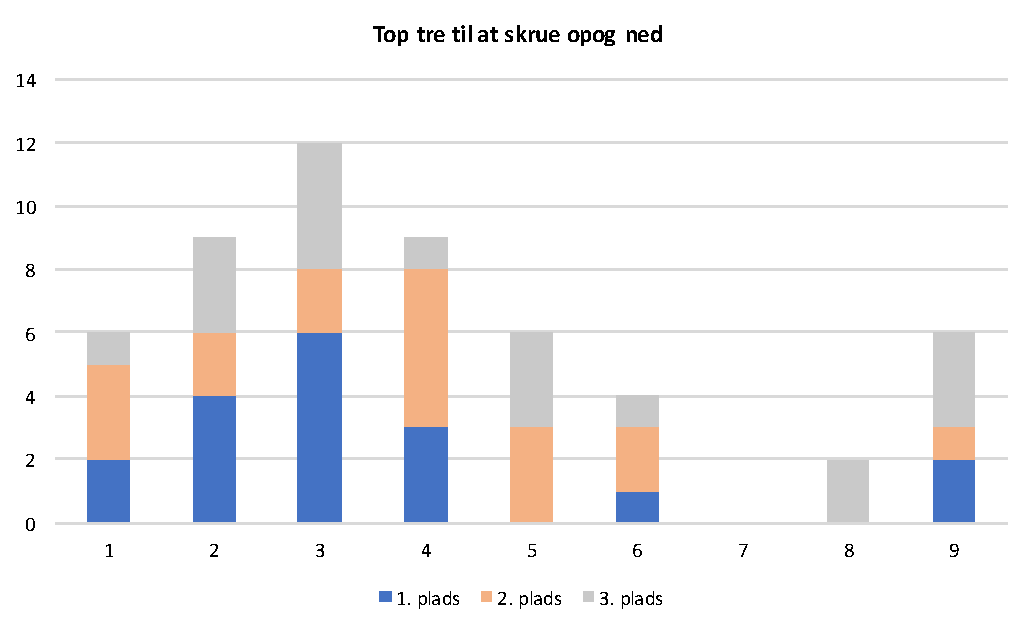
\includegraphics[resolution=300,width=0.9\textwidth]{Test1/DatabehandlingGrafer/TopTreVolumen}
	\caption{Barplot over hvordan hvert gestik-par indgår i testpersonernes top tre i forhold til at skrue op og ned.}
	\label{fig:SamletTopTreVolumen}
\end{figure}
\noindent
%
Da der er tre gestik-par, som er blevet ekskluderet, kan ovenstående  \autoref{tab:GestikParITopTreVolumen} med fordel opsummeres både i forhold til at fjerne de tre gestik-par men også i forhold til at opsummere hvor mange gange de fire tilbageværende gestik-par indgår i top tre rangeringen. 
%
\begin{table}[H]
	\centering
	\begin{tabular}{ | p{2.4cm} | p{2.4cm} | p{2.4cm} | p{2.4cm} |p{2.4cm}|}
		\hline
		& 1. Plads & 2. Plads & 3. Plads & I alt \\ \hline
		Gestik-par 1 & 2 & 3 & 1 & 6\\ \hline
		Gestik-par 2 & 4 & 2 & 3 & 9\\ \hline
		Gestik-par 3 & 6 & 2 & 4 & 12\\ \hline
		Gestik-par 4 & 3 & 5 & 1 & 9\\ \hline 
		Gestik-par 5 & 0 & 3 & 3 & 6\\ \hline
		Gestik-par 9 & 2 & 1 & 3 & 6\\ \hline
	\end{tabular}
	\caption{Oversigt over dels hvor mange gange hvert gestik-par indgår i samtlige testpersoners top tre i forbindelse med at ændre volumen og dels over hvor mange gange et gestik-par sammenlagt indgår i en top tre.}
	\label{tab:GestikParITopTrePauseVolumen}
\end{table}
\noindent
%